Fuzzy neurons are neurons that follows the basic idea of artificial neurons with small changes:

\begin{itemize}
\item The inputs to the fuzzy neurons $x_1, x_2, \dots, x_n$ represent fuzzy labels of fuzzy input variables,
\item The weights $w_i$ are replaced by functions $\mu_i$ which are the membership functions of the fuzzy labels $x_i \in (i = 1, 2, \dots, n)$,
\item Excitatory connections are represented by MIN operation and inhibitory connections by fuzzy logic complements followed by MIN operation,
\item Threshold level is not assigned.
\end{itemize}

In those fuzzy neurons learning is not present.
Membership functions attached to neuron connections are not changing.

\clearpage
To improve those traits of fuzzy neuron, Yamakwa et al. in 1992~\cite{yamakawa} came up with the idea of \emph{neo-fuzzy neurons} as a follow up to fuzzy neurons.
Those neurons differ to previously described fuzzy neurons in:

\begin{itemize}
\item Their inputs $x_1, x_2, \dots, x_n$ represent fuzzy variables,
\item In addition to the membership function $\mu_{ij}$ , which is bound to the input segment $x_{ij}$, weights $w_ij$ are also assigned, subject to a training procedure,
\item The segments $x_{i1}, x_{i2}, \dots, x_{il}$ have standard triangular membership functions; thus an input activates only two membership functions simultaneously; the sum of the degree to which an input value x'i belongs to any two neighboring membership functions $\mu_{ik}(x_i')$ and $\mu_{i,k+1}(x_i')$ is always equal to 1.
\end{itemize}

The model of neo-fuzzy neuron together with detailed diagram of its nodes and membership functions attached to its connection is depicted in Figure~\ref{fig:neuro_fuzzy_model}.

\begin{figure}[h!]
  \centering
	\captionsetup{width=24pc}
    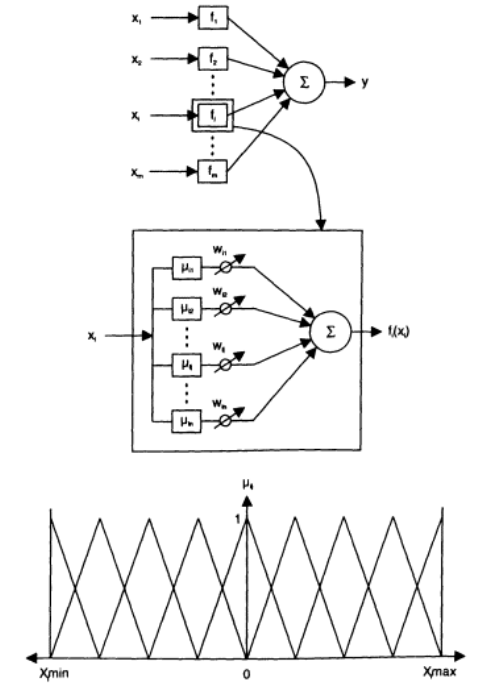
\includegraphics[width=0.55\textwidth]{images/neuro_fuzzy_model.png}
	\caption{Yamakawa's neo-fuzzy neuron. Each of the $m$ functions $f_i, i \in (1, 2, ..., m)$ bound to each of the $m$ inputs $x_i$ are represented by n = 9 fuzzy membership functions $T_ij$ , standard triangular ones uniformly distributed over the universe $Ux_i$ , as well as by corresponding weights $w_{ij}$ which are subject to change during training.}
	\label{fig:neuro_fuzzy_model}
\end{figure}